%! Author = amatarazzo
%! Date = 09/05/24

\chapter{Utilization Strategies and Techniques}
\label{ch:utilization}

\section{Introduction}
\label{sec:ch4-introduction}

In this chapter, we will discuss the strategies and techniques that can be used to utilize large language models effectively.
We will start by discussing the importance of context in utilizing large language models and how it can be used to improve their performance.
We will then move on to the concept of chain-of-thought prompting and how it can be used to guide the generation of text.
Finally, we will discuss the importance of planning for complex tasks and how it can be used to improve the performance of large language models.

\begin{table}[h!]
	\centering
	\tiny
	\begin{tabularx}{\textwidth}{|l|X|X|}
		\hline
		\textbf{Approach}                         & \textbf{Representative Work}                                                                                                                                                                                                                                                                                                                                                                                                                 & \textbf{Key Point}                                                                                                                                                                                                                                                                                                                                                                                                                                                                                                                                                                                                                                                                                                                                                                                                                                                          \\
		\hline
		\textbf{In-context Learning (ICL)}        & KATE~\cite{liu2022good}, EPR~\cite{rubin2022learning}, SG-ICL~\cite{kim2022self}, APE~\cite{zhou2023large}, Structured Prompting~\cite{hao2022structured}, GlobalE \& LocalE~\cite{lu2022fantastically}                                                                                                                                                                                                                                      & Demonstration selection (similar, k-NN) \newline Demonstration selection (dense retrieval; contrastive learning) \newline Demonstration selection (LLM as the demonstration generator) \newline Demonstration format (automatic generation \& selection) \newline Demonstration format (grouped context encoding; rescaled attention) \newline Demonstration order (entropy-based metric; probing set generation with LLM)                                                                                                                                                                                                                                                                                                                                                                                                                                                  \\
		\hline
		\textbf{Chain-of-thought Prompting (CoT)} & Complex CoT~\cite{fu2022complexity}, Auto-CoT~\cite{zhang2022automatic}, Selection-Inference~\cite{creswell2022selection}, Self-consistency~\cite{wang2022self}, DIVERSE~\cite{li2022making}, Rationale-augmented ensembles~\cite{wang2022rationale}                                                                                                                                                                                         & Demonstration (complexity-based selection) \newline Demonstration (automatic generation) \newline Generation (alternate between selection and inference) \newline Generation (diverse paths; self-ensemble) \newline Generation (diverse paths; Verification (step-wise voting)) \newline Generation (rationale sampling)                                                                                                                                                                                                                                                                                                                                                                                                                                                                                                                                                   \\
		\hline
		\textbf{Planning}                         & Least-to-most prompting~\cite{zhou2022least}, DECOMP~\cite{khot2022decomposed}, PS~\cite{wang2023plan}, Faithful CoT~\cite{lyu2023faithful}, PAL~\cite{gao2022pal}, HuggingGPT~\cite{shen2023hugginggpt}, AdaPlanner~\cite{sun2023adaplanner}, TIP~\cite{lu2023multimodal}, RAP~\cite{hao2023reasoning}, ChatCoT~\cite{chen2023chatcot}, ReAct~\cite{yao2022react}, Reflexion~\cite{shinn2023reflexion}, Tree of Thoughts~\cite{yao2023tree} & Plan generation (text-based; problem decomposition) \newline Plan generation (text-based; problem decomposition) \newline Plan generation (text-based) \newline Plan generation (code-based) \newline Plan generation (code-based; Python) \newline Plan generation (code-based; models from HuggingFace) \newline Plan refinement (skill memory) \newline Feedback acquisition (visual perception) \newline Feedback acquisition (LLM as the world model; Plan refinement (Monte Carlo Tree Search)) \newline Feedback acquisition (tool); Plan refinement (conversation between LLM and tools) \newline Feedback acquisition (tool); Plan refinement (synergizing reasoning and acting) \newline Feedback acquisition (text-based self-reflection); Plan refinement (dynamic memory) \newline Feedback acquisition (vote comparison); Plan refinement (tree-based search) \\
		\hline
	\end{tabularx}
	\caption{Typical LLM utilization methods and their key points for ICL, CoT, and planning. Note that the key points only highlight the most important technical contribution. Source: \textcite{survey}}
	\label{tab:utilization-methods}
\end{table}

\section{In-Context Learning}
\label{sec:in-context-learning}
In-context learning is a special prompting technique, initially introduced by \textcite{brown2020language}, that allows the model to learn from the context of the prompt (examples shown in Figure~\ref{fig:in-context-learning}).
\begin{figure}[h!]
	\centering
	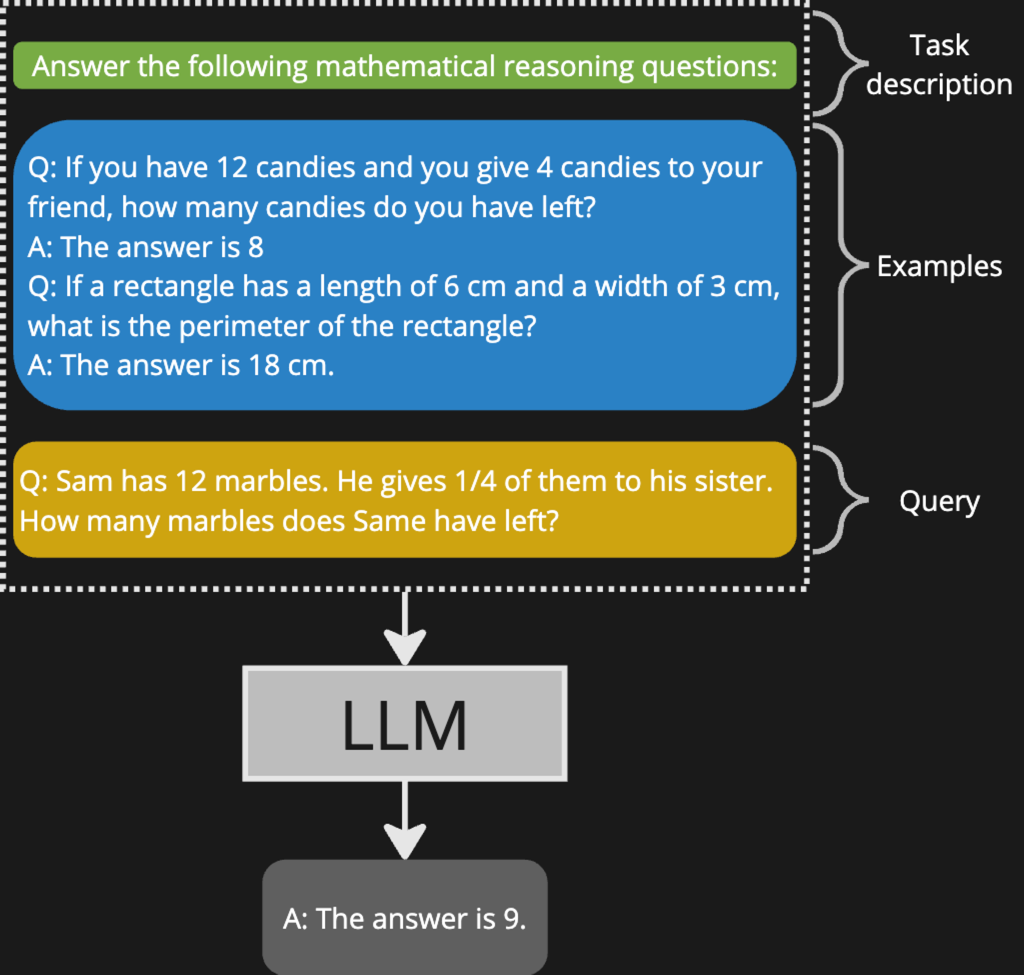
\includegraphics[width=\textwidth]{icl}
	\caption{In-context learning contrasted with traditional fine-tuning. Source: \textcite{brown2020language}}
	\label{fig:in-context-learning}
\end{figure}
ICT consists of the task description and/or few examples of the task as demonstrations combined in a specific order to form natural language prompts with specifically designed templates~\cite{brown2020language}.
Finally, the test instance is appended to the prompt to form the input for LLMs to generate the output.

Based on task demonstrations, LLMs can learn to perform a new task without explicit gradient update.
Formally, the in-context learning task can be defined as follows:
\begin{equation}
	LLM(I, \underbrace{f(x_1, y_1), \dots, f(x_k, y_k)}_\text{demonstrations}, \underbrace{f(x_{k+1}}_\text{input}, \underbrace{\uline{~~~}}_\text{answer})) \rightarrow \hat{y}_{k+1}
	\label{eq:ict}
\end{equation}
where $I$ is a task description, $f(x_i, y_i)$ function that convert task demonstration to natural language, $x_{k+1}$ is a new input query, $\hat{y}_{k+1}$ is the prediction of the output generated, and the actual answer $y_{k+1}$ is left as a blank to be predicted by the LLM\@.

\begin{figure}[h!]
	\centering
	\resizebox{\textwidth}{!}{
		\begin{forest}
			forked edges,
			for tree={
					grow=east,
					reversed=true, % reverse the direction of growth
					anchor=base west, % align text to the west
					parent anchor=east,
					child anchor=west,
					base=left,
					font=\small,
					rectangle,
					draw,
					align=left,
					s sep=3mm, % sibling distance
					l sep=10mm, % level distance
					inner xsep=3mm, % text padding horizontal
					inner ysep=1mm  % text padding vertical
				}
				[In-context Learning
						[Inference
								[Scoring Function
										[{Channel prompt tuning~\cite{min2022metaicl},\\
													kNN-Prompting~\cite{xu2023knn}}]
								]
								[Demonstration Designing
										[Organization
												[Selecting
														[{KATE~\cite{liu2022good}, \\
																	EPR~\cite{rubin2022learning}, \\
																	PPL~\cite{gonen2022demystifying}, \\
																	SG-ICL~\cite{kim2022self}, \\
																	Self Adaptive~\cite{wu2022selfadaptive}, \\
																	MI~\cite{sorensen2022information}, \\
																	Q-Learning~\cite{zhang2022active}, \\
																	Informative Score~\cite{li2023finding}, \\
																	Topic~\cite{wang2023large}, \\
																	UDR~\cite{li2023finding}}]
												]
												[Ordering
														[{GlobalE\&LocalE~\cite{lu2022fantastically}}]
												]
										]
										[Formatting
												[Instruction
														[{Instruction Induction~\cite{honovich2022instruction}, \\
																	APE~\cite{zhou2022least}, \\
																	Self-Instruct~\cite{wang2022selfinstruct}}]
												]
												[Reasoning Steps
														[{CoT~\cite{wang2022selfinstruct}, \\
																	Complex CoT~\cite{fu2022complexity}, \\
																	AutoCoT~\cite{zhang2022automatic}, \\
																	Self-Ask~\cite{press2022train}, \\
																	MoT~\cite{li2023mot}, \\
																	SuperICL~\cite{xu2023small}, \\
																	iCAP~\cite{wang2022iteratively}, \\
																	Least-to-Most Prompting~\cite{zhou2022least} }]
												]
										]
								]
						]
						[Training
								[Warmup
										[Self-supervised In-context Training
												[{Self-supervised ICL~\cite{chen2022improving}, \\
															PICL~\cite{gu2023pretraining}}]
										]
										[Supervised In-context Training
												[{MetaICL~\cite{min2022metaicl}, \\
															OPT-IML~\cite{iyer2022opt}, \\
															FLAN~\cite{wei2022fine}, \\
															Super-NaturalInstructions~\cite{wang2022super}, \\
															Scaling Instruction~\cite{chung2022scaling}, \\
															Symbol Tuning~\cite{wei2023symbol}}]
										]
								]
						]
				]
		\end{forest}
	}
	\caption{Taxonomy of in-context learning. The training and the inference stage are two main stages for ICL. During the training stage, existing ICL studies mainly take a pretrained LLM as backbone, and optionally warmup the model to strengthen and generalize the ICL ability. Towards the inference stage, the demonstration designing and the scoring function selecting are crucial for the ultimate performance. Source: \textcite{dong2023survey}}
	\label{fig:icl-taxonomy}
\end{figure}

Since the performance of ICL heavily relies on demonstrations, it is important to properly design them in the prompts.
The tree main aspects are a direct consequence of what defined in the the Equation~\ref{eq:ict}: how to select the task demonstrations, how to convert them into natural language, and arrange demonstrations in a reasonable order.

Different training strategies enhance ICL capabilities, improving performance across various tasks without specific task optimization during the pre-training phase (see Figure~\ref{fig:icl-taxonomy} under the Training branch).
Main approaches include Supervised In-context Training, such as MetaICL\footnote{Meta-training for InContext Learning} and Symbol Tuning, and Self-supervised In-context Training, such as Self-supervised ICL and PICL~\cite{dong2023survey}.

MetaICL~\cite{min2022metaicl} proposed to continually train LLMs on a wide range of tasks\footnote{Classification, question answering,
	natural language inference, paraphrase detection and more} with demonstration examples.
This approach is related to other works that uses multi-task learning for better zero-shot performance at test time~\cite{min2022metaicl}.
However, MetaICL is distinct as it allows learning new tasks from k examples alone, without relying on a task reformatting (e.g., reducing everything to question answering)
or task-specific templates (e.g., converting different tasks to a language modeling problem).
MetaICL is based on the core idea of in-context learning by conditioning on training examples (i.e., explicitly training on an in-context learning objective).

Symbol Tuning~\cite{wei2023symbol} instead fine-tunes language models on in-context input-label pairs, substituting natural language labels (e.g., "positive/negative sentiment") with arbitrary symbols (e.g., "foo/bar").
As a result, symbol tuning demonstrates an enhanced capacity to utilize in-context information for overriding prior semantic knowledge.
Compared to MetaICL, which constructs several demonstration examples for each task, instruction tuning mainly considers an explanation of the task and is more easier to scale up.

Self-supervised ICL leverages raw corpora to generate input/output pairs as training data, while PICL also utilizes raw corpora but employs a simple language modeling objective, promoting task inference and execution based on context.
PICL shown to be more effective in zero-shot settings and tasks generalization~\cite{dong2023survey}.

Effective demonstration design is crucial, involving selecting and ordering examples, or using instruction induction and reasoning steps (as shown in Figure~\ref{fig:icl-taxonomy} under the Inference/ Demonstration Designing branch).
The selection aims to choose good examples for ICL using unsupervised\footnote{Based on pre-defined metrics} or supervised methods.
For example, KATE~\cite{liu2022good} and EPR~\cite{rubin2022learning} select demonstrations based on similarity.
The ordering of the selected demonstrations is also an important aspect of demonstration design.
\textcite{lu2022fantastically} have proven that order sensitivity is a common problem and affects various models.
To handle this problem, studies have proposed several training-free methods to order demonstrations.
\textcite{liu2022good} sorted examples based on similarity, while GlobalE\&LocalE~\cite{lu2022fantastically} orders demonstrations based on global and local entropy.

A common representation of demonstrations is concatenating examples $(x_1, y_1), \cdots, (x_k, y_k)$ with a template T directly.
However, this approach may not be optimal for all tasks, i.e.\ when the task is complex or requires multiple steps such as math word problems and common-sense reasoning.
In those cases, it's not easy to learn the mapping from $x_i$ to $y_i$ with only $k$ demonstrations.
Template engineering has been studied in \textcite{liu2021pretrain, liu2022good} to generate task-specific templates.
Some researches have proposed to design a better format of demonstrations, by describing tasks with instructions I and adding intermediate reasoning steps between examples $(x_i, y_i)$.
Instructions depends heavily on human input, but they can be generated automatically as shown in \textcite{honovich2022instruction} given several demonstration examples.
\textcite{zhou2023large} proposed APE for automatic instruction generation and selection.
To further improve the quality of the automatically generated instructions, \textcite{wang2022selfinstruct} proposed Self-Instruct, which is able to get rid of its own generations.

The approach of adding intermediate reasoning steps between examples introduced in \textcite{wang2023large} is also called Chain-of-Thought prompting.
We will delve into Chain-of-Thought prompting in the next Section~\ref{sec:chain-of-thought}.

At the inference stage, ICL operates without explicit updates, focusing on task recognition and learning through demonstrations.
Task recognition utilizes pre-trained knowledge to solve tasks identified in the demonstrations.
A Probably Approximately Correct (PAC)~\cite{wies2023learnability} framework has been proposed to evaluate ICL’s learnability, suggesting that LLMs can recognize tasks from minimal inputs.

Task learning, on the other hand, involves LLMs learning new tasks through demonstrations, akin to implicit fine-tuning through the attention mechanism, which generates meta-gradients.
With the examples provided in ICL, LLMs can implement learning algorithms such as gradient descent or directly compute the closed-form solution to update these models during forward computation.
Under this explanation framework, it has been shown that LLMs can effectively learn simple linear functions and even some complex functions like decision trees with ICL~\cite{akyurek2022what}.
Different model scales exhibit distinct capabilities; smaller models are adept at task recognition, while larger models (at least 66 billion parameters) are necessary for task learning~\cite{pan2023what}.

\begin{table}[h!]
	\centering
	\small
	\begin{tabularx}{0.8\textwidth}{lXccc}
		\toprule
		\textbf{Scoring Function} & \textbf{Target}              & \textbf{Efficiency} & \textbf{Task Coverage} & \textbf{Stability} \\
		\midrule
		Direct                    & $\mathcal{M}(y_j \mid C, x)$ & +++                 & +                      & +                  \\
		PPL                       & PPL($S_j$)                   & +                   & +++                    & +                  \\
		Channel                   & $\mathcal{M}(x \mid C, y_j)$ & +                   & +                      & ++                 \\
		\bottomrule
	\end{tabularx}
	\caption{Summary of different scoring functions.}
	\label{tab:scoring-functions}
\end{table}

The last piece of ICL is the scoring function, which decides how to transform the predictions of the LLMs into an estimation of the likelihood of a specific answer.
A direct estimation method adopts the conditional probability of candidate answers and select the higher probability as the final answer~\cite{brown2020language}.
However, this method poses some restrictions on the template design, e.g., the answer tokens should be placed at the end of input sequences.
Perplexity (PPL) is another commonly-used metric that computes the PPL of the entire input sequence:
\begin{equation}
	S_j = \{C,s(x,y_i,I)\}
	\label{eq:ppl}
\end{equation}
where C are the tokens of the demonstration examples, $x$ is the input query, and $y_i$ is the candidate label.
As PPL is a global metric (i.e., it considers the entire input sequence), it removes the limitations of token positions but requires extra computation time.
In generation tasks such as machine translation, ICL predicts the answer by decoding tokens with the highest sentence probability combined with diversity-promoting strategies such as beam search or Top-p and Top-k~\cite{holzman2020curious} sampling algorithms.
\textcite{min2022noisy} proposed a channel scoring function that estimates the likelihood of the input query given the candidate answer\footnote{Compute the conditional
	probability in a reversed direction}, which is more efficient and stable than the direct estimation method.
In this way language models are required to generate every token in the input, which could boost the performance under imbalanced training data regimes.
To calibrate the bias or mitigate the sensitivity via scoring strategies some studies add additional calibration parameters to adjust the model predictions~\cite{zhao2021calibrate}.

\subsection{ICL performance and origins}
\label{subsec:icl-performance}

Knowing and understanding the factors that influence ICL can help to improve the performance of LLMs.
ICL has a close connection with instruction tuning (discussed in Section~\ref{subsec:instruction-tuning}) in that both utilize natural language to format the task or instances.
However, instruction tuning needs to fine-tune LLMs for adaptation, while ICL only prompts LLMs for utilization~\cite{survey}.
Furthermore, instruction tuning can enhance the ICL ability of LLMs to perform target tasks, especially in the zero-shot setting\footnote{Using only task descriptions}~\cite{chung2022scaling}.

\begin{table}[h!]
	\centering
	\small
	\begin{tabularx}{0.8\textwidth}{lX}
		\toprule
		\textbf{Stage} & \textbf{Factor}                                                                               \\
		\midrule
		\multirow{4}{*}{Pretraining}
		               & Pretraining corpus domain~\cite{shin2022effect}                                               \\
		               & Pretraining corpus combination~\cite{shin2022effect}                                          \\
		               & Number of model parameters~\cite{wei2022emergent, brown2020language}                          \\
		               & Number of pretraining steps~\cite{wei2022emergent}                                            \\
		\midrule
		\multirow{8}{*}{Inference}
		               & Label space exposure~\cite{min2022rethinking}                                                 \\
		               & Demonstration input distribution~\cite{min2022rethinking}                                     \\
		               & Format of input-label pairing~\cite{min2022rethinking,an2023how}                              \\
		               & Demonstration input-label mapping~\cite{min2022rethinking, yoo2022groundtruth, wei2023symbol} \\
		               & Demonstration sample ordering~\cite{lu2022fantastically}                                      \\
		               & Demonstration-query similarity~\cite{lu2022fantastically}                                     \\
		               & Demonstration diversity~\cite{an2023how}                                                      \\
		               & Demonstration complexity~\cite{an2023how}                                                     \\
		\bottomrule
	\end{tabularx}
	\caption{Summary of factors that have a relatively strong correlation to ICL performance. Source: \textcite{dong2023survey}}
	\label{tab:icl-factors}
\end{table}

There are several factors that have a relatively strong correlation to ICL performance, as shown in Table~\ref{tab:icl-factors}.
ICL ability may give raise putting multiple corpora together in the pre-training stage, and the domain source is more important than the corpus size~\cite{shin2022effect}, while pretrain on corpora related to downstream tasks and models with lower perplexity do not always perform better in ICL~\cite{shin2022effect}.
\textcite{wei2022emergent} suggested that a pretrained model suddenly acquires some emergent ICL abilities when it achieves a large scale of pretraining steps or model parameters and \textcite{brown2020language} showed that the ICL ability grows as the parameters of LLMs increase from 0.1 billion to 175 billion.
At inference stage, the properties of the demonstrations influence the ICL performance, such as the label space exposure, the format of input-label pairing, the ordering of demonstration samples, and the complexity of demonstrations~\cite{min2022rethinking, an2023how, lu2022fantastically}.
There are contrasting results on the impact of input-label mapping related to ICL~\cite{min2022rethinking, yoo2022groundtruth}.
An interesting finding is that, when a model is large enough, it will show an emergent ability to learn input-label mappings, even if the labels are flipped\footnote{Flipped-label ICL uses flipped targets, forcing the model override semantic priors in order to follow the in-context exemplars. For example, in sentiment analysis task, the label "Positive" become "Negative" in ICL context and viceversa} or semantically-unrelated\footnote{The labels are semantically unrelated to the task(e.g., for sentiment analysis, it uses “foo/bar” instead of “negative/positive”)}~\cite{wei2023larger}.
Some general validated factors for the ICL demonstrations are that they should be diverse, simple, and similar to the test example in terms of the structure~\cite{an2023how}.
\textcite{lu2022fantastically} indicated that the demonstration sample order is also an important factor.
\textcite{liu2022good} found that the demonstration samples that have closer embeddings to the query samples usually bring better performance than those with farther embeddings.

The reasons for the ICL ability has been investigated from different perspectives.
Focusing on the pretraining data distribution, \textcite{chan2022data} showed that the ICL ability is driven by data distributional properties.
The ICL ability emerges when the training data have examples appearing in clusters and have enough rare classes.
\textcite{xie2022an} explained ICL as implicit Bayesian inference and constructed a synthetic dataset to prove that the ICL ability emerges when the pretraining distribution follows a mixture of hidden Markov models.
Under the learning mechanism, the ICL ability is explained by ability of Transformers to encode effective learning algorithms to learn unseen linear functions according to demonstration samples, and encoded learning algorithms can achieve a comparable error to that from a least squares estimator~\cite{garg2023transformers}.
Also \textcite{li2023transformers} showed the ability of Transformers to implement a proper function class through implicit empirical risk minimization for the demonstrations.
From an information-theoretic perspective, \textcite{hahn2023theory} showed an error bound for ICL under linguistically motivated assumptions to explain how next-token prediction can bring about the ICL ability.
Another series of works attempted to build connections between ICL and gradient descent and found that Transformer-based in-context learners can implement standard finetuning algorithms implicitly~\cite{akyurek2022what, vonoswald2023transformers, li2023transformers}.
Looking at functional components, \textcite{olsson2022incontext} found indirect evidence that "Induction heads"\footnote{attention heads that implement a simple algorithm to complete token sequences like $[A][B] \dots [A] \Rightarrow [B]$} might constitute the mechanism for the majority of all ICL in large transformer models.

In-context learning (ICL) evaluation spans traditional tasks and newly proposed challenging tasks, as well as providing open-source tools for standardized evaluation.
ICL has been tested against established benchmarks such as SuperGLUE and SQuAD, with mixed results.
GPT-3, for example, exhibited comparable performance to state-of-the-art fine-tuning on some tasks within SuperGLUE but lagged in most natural language understanding tasks.
Scaling the number of demonstration examples has shown potential but has yet to bridge the gap fully between ICL and traditional fine-tuning methods~\cite{brown2020language, hao2022structured}.

To assess the capabilities of large language models (LLMs) beyond traditional finetuning, new benchmarks have been introduced.
The BIG-Bench and BIG-Bench Hard focus on tasks ranging from linguistics to social behaviors, with models outperforming human raters on many of these tasks~\cite{srivastava2023imitation, suzgun2022challenging}.
OPT-IML Bench has been designed to evaluate the generalization capabilities of LLMs across various held-out categories, emphasizing the model's generalization capabilities~\cite{iyer2022opt}.
OpenICL has been developed to provide a flexible and unified framework for ICL evaluation.
This toolkit supports different LLMs and tasks, enabling consistent implementation and evaluation of ICL methods across various studies~\cite{wu2023openicl}.

The application of In-Context Learning (ICL) has transcended the domain of natural language processing (NLP), influencing research in various modalities such as visual tasks, vision+language integration, and speech.
Visual In-Context Learning explores how models generalize learned visual concepts to new, unseen tasks by leveraging contextual demonstrations in a manner akin to NLP-based ICL. Techniques such as image patch infilling and the training of models like masked autoencoders (MAE) exemplify this approach~\cite{bar2022visual}.
Noteworthy models like Painter and SegGPT have been developed to handle multiple tasks or integrate various segmentation tasks into a single framework~\cite{wang2023images, wang2023seggpt}.
The Prompt Diffusion model introduced by \textcite{wang2023incontext} represents a pioneering effort in diffusion-based models displaying ICL capabilities, particularly when guided by textual prompts~\cite{wang2023incontext} .
In the realm of vision-language tasks, the integration of visual contexts with linguistic models has led to significant advancements.
Models such as Frozen and Flamingo have demonstrated the feasibility of multi-modal few-shot learning by combining vision encoders with large language models (LLMs).
These models effectively perform ICL on multi-modal tasks when trained on large-scale multi-modal web corpora~\cite{tsimpoukelli2021frozen, alayrac2022flamingo}.
Kosmos-1 and METALM further extend these capabilities by demonstrating strong performance across various vision-language tasks, underpinned by a semi-causal language modeling objective~\cite{huang2023language, hao2022language} .

\subsection{ICL future research}
\label{subsec:icl-future}

Future research in ICL is expected to focus on several key areas, including the optimization of pretraining objectives, the distillation of ICL abilities, the enhancement of ICL robustness, the improvement of ICL efficiency and scalability, the updating of knowledge within LLMs, the augmentation of models, and the expansion of ICL into multi-modal domains~\cite{dong2023survey}.
Optimizing pretraining objectives to better align with ICL requirements could enhance model capabilities for ICL applications.
Introducing intermediate tuning phases and tailoring pretraining objectives to better align with ICL requirements could bridge this gap and enhance model capabilities for ICL applications~\cite{shin2022effect}.
On important goal is to be able to distill ICL capabilities from larger models to smaller, more efficient models, potentially enabling the deployment of ICL in resource-constrained environments~\cite{magister2022teaching}.
Another area of improvement is the robustness of ICL, which is highly susceptible to the format and permutation of demonstrations~\cite{zhao2021calibrate, lu2022fantastically}, without compromising accuracy or efficiency~\cite{chen2024relation}.

A more theoretical understanding of ICL's mechanisms could lead to more robust implementations.
Moreover the scalability of ICL is constrained by the input limitations of language models and the computational cost associated with large numbers of demonstrations.
Innovative strategies like structured prompting~\cite{hao2022structured} and dynamic prompting~\cite{wang2023efficient} are being explored to address these challenges.
The development of models with extended context capabilities~\cite{li2023contextual} indicates significant potential for progress in this area.
Finally, the expansion of ICL into multi-modal domains is expected to yield new insights and applications, particularly in the fields of vision and speech~\cite{dong2023survey}.


\section{Chain-of-Thought prompting}
\label{sec:chain-of-thought}

Chain-of-Thought (CoT) prompting is an enhanced strategy developed to augment the performance of large language models (LLMs) on complex reasoning tasks such as arithmetic, commonsense, and symbolic reasoning~\cite{wei2022chain, miao2021diverse, talmor2019commonsenseqa}.
This method integrates intermediate reasoning steps within the prompts, thereby providing a more structured path towards the solution.
\begin{figure}[h!]
	\centering
	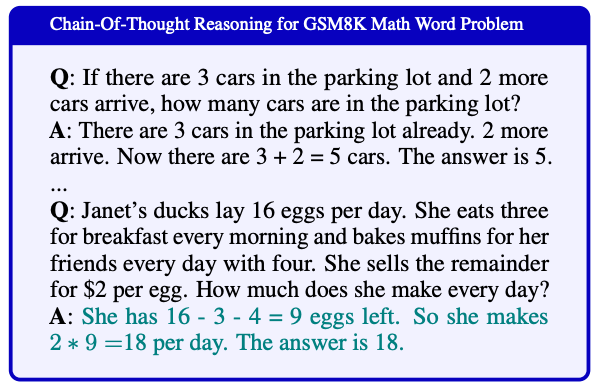
\includegraphics[width=0.6\textwidth]{cot-reasoning}
	\caption{Chain-of-Thought reasoning for GSM8K math word problem. The prompt is colored black and the reasoning path produced by the language model is colored teal. This reasoning path contains two reasoning steps. Source: \textcite{li2022making}}
	\label{fig:cot-reasoning}
\end{figure}
To some extent, CoT can be considered a special case of ICL, as it involves the generation of prompts with a series of intermediate reasoning steps (Figure~\ref{fig:chain-of-thought}), but the ordering of demonstrations in this case has a s relatively minor impact on the performance of LLMs~\cite{wei2022chain}.

\textcite{wei2022chain, wang2022self} have shown that language models, when large enough (i.e., \textgreater 100 billion parameters), can learn to perform complex reasoning tasks through CoT prompting without explicit task-specific~\cite{wei2022emergent}.

\begin{figure}[h!]
	\centering
	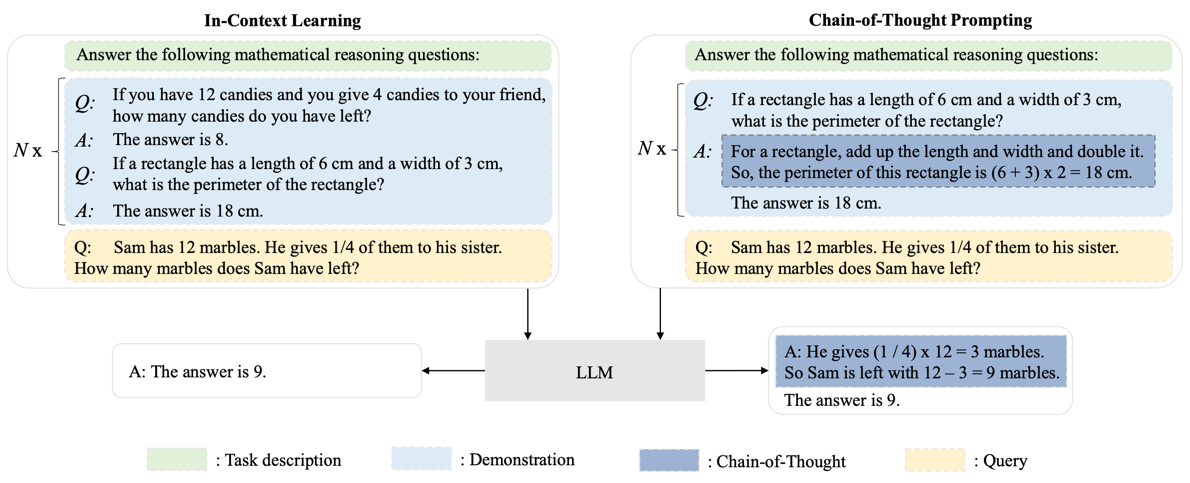
\includegraphics[width=\textwidth]{icl-vs-cot}
	\caption{A comparative illustration of in-context learning (ICL) and chain-of-thought (CoT) prompting. ICL prompts LLMs with a natural language description, several demonstrations, and a test query, while CoT prompting involves a series of intermediate reasoning steps in prompts. Source: \textcite{survey}}
	\label{fig:chain-of-thought}
\end{figure}

CoT can be effectively combined with In-context Learning (ICL) in both few-shot and zero-shot settings:
\begin{itemize}
	\item \textbf{Few-shot CoT.} {In the few-shot scenario, CoT augments standard input-output pairs with intermediate reasoning steps.
		      The design of CoT prompts is crucial; incorporating diverse and complex reasoning paths has been shown to significantly boost LLM performance.
		      An automated approach, Auto-CoT, facilitates the generation of CoT sequences without manual effort by clustering and selecting representative questions~\cite{zhang2022automatic}.
	      }
	\item \textbf{Zero-shot CoT.} {Unlike its few-shot counterpart, zero-shot CoT does not rely on annotated demonstrations.
		      Instead, it generates reasoning steps directly from a prompt, significantly improving performance when scaled to larger models.
		      This approach was pioneered by models like Flan-T5, which demonstrated improved zero-shot performance through instruction tuning on CoT annotations~\cite{chung2022scaling}.
	      }
\end{itemize}

\begin{figure}[h!]
	\centering
	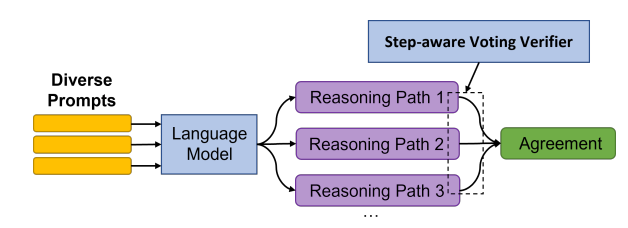
\includegraphics[width=0.6\textwidth]{diverse}
	\caption{The DIVERSE approach for CoT. Source: \textcite{li2022making}}
	\label{fig:diverse}
\end{figure}

To apply these strategies effectively, it is essential to design CoT prompts that guide the model through the reasoning process.
In \textcite{li2022making}, the authors have shown that using diverse CoTs (i.e., prompts with multiple reasoning paths for each problem) can significantly enhance the performance of LLMs on complex reasoning tasks.
The proposed method, DIVERSE\footnote{\textbf{Di}verse \textbf{Ve}rifier on \textbf{R}easoning \textbf{S}t\textbf{e}p}, generates diverse CoTs by leveraging a self-ensemble approach that alternates between selection and inference.
It has three main components: first, it generates diverse prompts to explore different reasoning paths for the same question; second, it uses a verifier to filter out incorrect answers based on a weighted voting scheme; and third, it verifies each reasoning step individually instead of the whole chain (Figure ~\ref{fig:diverse}).
In the first step, the model generates multiple reasoning paths for each question, which are then used to generate diverse prompts following the idea that \textit{"All roads lead to Rome"}.
As improvement of \textcite{wang2022self}, DIVERSE selects $M_1$ different prompts for each question, and $M_2$ reasoning paths for each prompt, resulting in $M_1 \times M_2$ diverse prompts.
Then the verifier takes a question and a candidate reasoning path, and outputs the probability of the reasoning path leads to the correct answer.
Different predictions are aggregated using a \textit{voting verifier} to obtain the final prediction:
\begin{equation}
	\hat{y} = \underset{y}{\text{arg max}} \sum_{i=1}^{M_1} \textbf{1}_{y = y_{i}} \cdot f(\textbf{x}_i, \textbf{z}_i, \textbf{y}_i)
	\label{eq:diverse}
\end{equation}
where $\textbf{1}_{y = y_{i}}$ is an indicator function that equals 1 if $y = y_{i}$, and $f(\cdot)$ is the probability produced by the verifier.

\begin{figure}[h!]
	\centering
	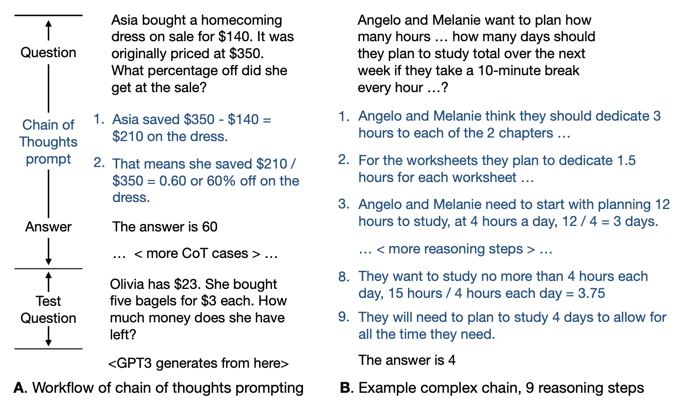
\includegraphics[width=0.8\textwidth]{cot-complex-chain}
	\caption{\textbf{A}: Chain of thoughts (in blue) are intermediate reasoning steps towards a final answer. The input of CoT prompting is a stack of few (often 8) CoT cases before a test question. Then the language model will continue generating an output CoT for the test question. \textbf{B}: Chains of harder reasoning complexity are chains with more reasoning steps (9 steps in this case, v.s. only 2 steps in subfigure A) .Source: \textcite{fu2022complexity}}
	\label{fig:cot-complex-chain}
\end{figure}

Another intuitive idea is that prompting with more complex reasoning steps (i.e., chains with more reasoning steps) are more likely to eliciting the reasoning ability of LLMs~\cite{fu2022complexity}, which can result in generating correct answers (Figure~\ref{fig:cot-complex-chain}).
There are other complexity indicators than the number of reasoning steps, such as question lengths or the length of underlying formula for solving a given problem but improvements of the performance are consistent across various complexity indicators.
Consequently, for datasets not annotated with reasoning steps, questions length can be used as a proxy for complexity to generate CoT prompts.
In that way is possible to annotate only the identified few-shot instances, thus reducing the annotation cost~\cite{fu2022complexity}.
To exclude complexity correlated factors, \textcite{fu2022complexity} proposed prompts evaluation:
\begin{itemize}
	\item \textbf{Simpler examples but the same total number of reasoning steps.} {For instance, comparing 24 cases that each require 3 reasoning steps with 8 cases that each require 9 reasoning steps, both resulting in a total of 72 steps.}
	\item \textbf{Prompts of the longest lengths but not necessarily the most steps.} {This ensures that the length itself is not the only factor being assessed.}
\end{itemize}
It turned out that the complexity of reasoning steps is the most important factor for the performance of LLMs on complex reasoning tasks~\cite{fu2022complexity}.
\begin{figure}[h!]
	\centering
	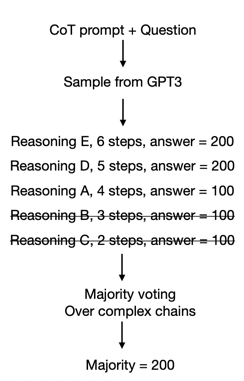
\includegraphics[width=0.2\textwidth]{cot-complexity}
	\caption{Complexity-based Consistency for CoT. During decoding, it sample N reasoning chains from the language model (N = 5 here), and take the majority answer over the K (K = 3 here) most complex generated chains. Source: \textcite{fu2022complexity}}
	\label{fig:complexity}
\end{figure}
Complexity based prompting can be further enhanced by using the output selection method called Complexity-based Consistency alleviating the possibility that model can take shortcuts during reasoning\footnote{Relying on spurious correlations that inevitably exist in the training data and are not related to the reasoning process as shown by \textcite{mudrakarta2018model, li2021why, sugawara2018makes}}.
The method explicitly promote outputs with more complex reasoning chains at inference time, similarly to the self-consistency practice in \textcite{wang2022self}.
A voting mechanism is used to select the final output among top K complex reasoning chains as shown in Figure~\ref{fig:complexity}.

\begin{figure}[h!]
	\centering
	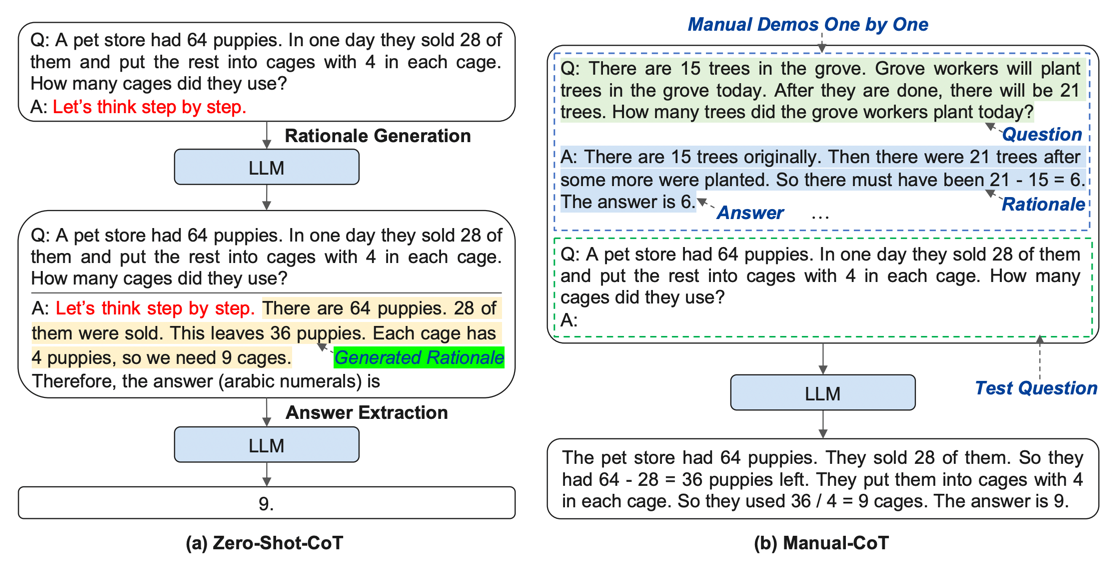
\includegraphics[width=\textwidth]{cot-zero}
	\caption{Zero-Shot-CoT~\cite{kojima2023large} (using the "Let’s think step by step" prompt) and Manual-CoT\cite{wei2022chain} (using manually designed demonstrations one by one) with example inputs and outputs of an LLM. Source: \textcite{zhang2022automatic}}
	\label{fig:zero-shot-cot}
\end{figure}

Previously mentioned methods rely on two major paradigms: Zero-Shot-CoT and Manual-CoT\@.
Zero-Shot-CoT is a task-agnostic paradigm that generates reasoning steps directly from the prompt, eliminating the need for annotated CoT datasets~\cite{kojima2023large}, adding a single prompt like "Let’s think step by step" after the test question to facilitate the reasoning chains in LLMs.
On the other hand, Manual-CoT uses manually designed demonstrations one by one, which can be expensive and time-consuming to create~\cite{wei2022chain}.
Since this prompting paradigm is task-agnostic and does not need input-output demonstrations, it is called Zero-Shot-CoT (left of Figure~\ref{fig:zero-shot-cot}).
With Zero-Shot-CoT, LLMs have shown to be decent zero-shot reasoners.

The other paradigm is few-shot prompting with manual reasoning demonstrations one by one~\cite{wei2022chain}.
Each demonstration has a question and a reasoning chain.
A reasoning chain is composed of a rationale (a series of intermediate reasoning steps) and an expected answer.
With all the demonstrations being manually designed, this paradigm is referred to as Manual-CoT (right of Figure~\ref{fig:zero-shot-cot}).

To mitigate the effect of reasoning chain mistakes from Zero-Shot-CoT, \textcite{zhang2022automatic} proposed the use of Auto-CoT, a method that generates demonstrations automatically, since their diversity is crucial for the performance of LLMs.
It consists of two main components: a clustering algorithm that groups similar questions together and a representative selection algorithm that selects the most representative questions from each cluster.
The overall procedure is illustrated in Figure~\ref{fig:auto-cot}.
\begin{figure}[h!]
	\centering
	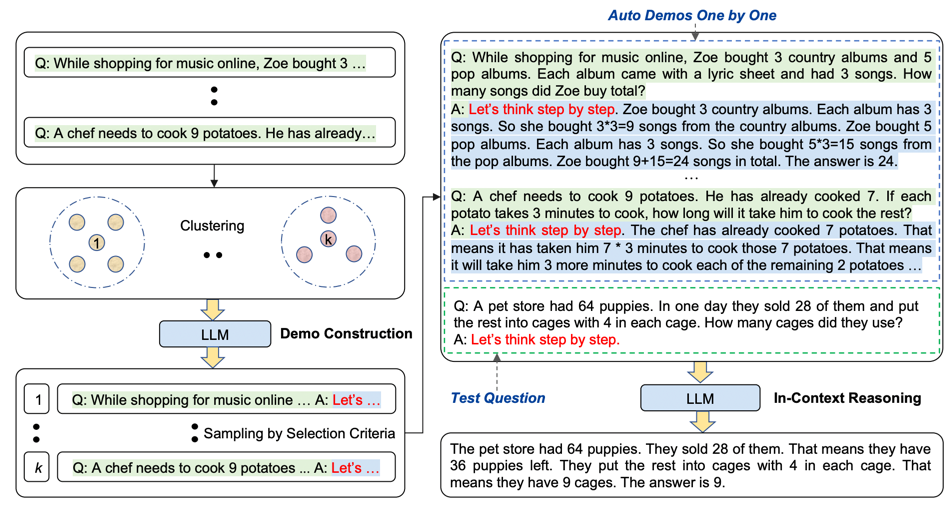
\includegraphics[width=\textwidth]{auto-cot}
	\caption{demonstrations (on the right) are automatically constructed one by one (total: k) using an LLM with the “Let’s think step by step” prompt. Source: \textcite{zhang2022automatic}}
	\label{fig:auto-cot}
\end{figure}
Diversity-based clustering may mitigate misleading by similarity effects\footnote{The retrieved demonstration questions are similar to the test question and asking "how long will it take him to cook \underline{the rest}?" The reasoning chains generated by Zero-Shot-CoT produce answers regarding "the total of" instead of "the rest". Following the demonstrations, the component the retrieves the top-k similar questions -- called Retrieval-Q-CoT -- also fails by misunderstanding the meaning of "the rest".}, and the representative selection algorithm can select the most representative questions from each cluster, are used as demonstrations to generate reasoning chains for the test question.
Auto-CoT has shown to be effective in generating diverse reasoning chains and improving the performance of LLMs on arithmetic and symbolic reasoning~\cite{zhang2022automatic}.

\subsection{CoT performance and origins}
\label{subsec:cot-performance}

CoT is an emergent ability~\cite{wei2022emergent}, so it has positive effects only on the performance of LLMs (>10 billion parameters) but not on smaller models.
Moreover CoT is only effective for tasks that requires step-by-step reasoning, such as arithmetic, commonsense, and symbolic reasoning~\cite{wei2022chain, miao2021diverse, talmor2019commonsenseqa}.
Whereas, for other tasks CoT can be detrimental to the performance of LLMs respect to standard prompting~\cite{wang2022rationale}, e.g., MNLI-m/mm, SST-2, and QQP from GLUE\cite{wang2018glue}.
It seems that the effectiveness of CoT is inversely proportional to the effectiveness of standard prompting~\cite{wei2022chain}.
Main prompting components, e.g., symbols, patterns, and text, have an impact on CoT.
It has been shown that pattern and text are essential for CoT performance, and removing them can lead to a significant drop in performance: text helps LLMs
to generate useful patterns, and patterns aid LLMs to understand tasks and generate texts that help solve them~\cite{madaan2022text}.

The origins of CoT ability is widely hypothesized to be elicited by training on code, since those models have shown to be more effective in reasoning tasks~\cite{fu2022gptroadmap, liang2022holistic}.
Intuitively, code data is well organized with algorithmic logic and programming flow,which may be useful to improve the reasoning performance of LLMs. However, this hypothesis still lacks publicly reported evidence of ablation experiments (with and without training on code).
We'll try to address this gap in the next chapter~\ref{ch:capabilities}, by conducting a series of experiments to evaluate the effectiveness of training on code data for reasoning tasks.
In addition, instruction tuning seems not to be the main factor for CoT ability, since the performance of LLMs on CoT tasks is not significantly improved by instruction tuning~\cite{chung2022scaling}.

\section{Planning for complex tasks}
\label{sec:planning}

ICL and CoT are two simple yet general strategies to solving various tasks.
However, they struggles with complex tasks that require long-term planning, such as mathematical word problems~\cite{qian2022limitations} and multi-hop question answering~\cite{bian2024chatgpt}.
In particular, \textcite{bian2024chatgpt} have shown that ChatGPT's ability to handle commonsense knowledge across various domains.
Commonsense knowledge\footnote{It includes knowledge about the spatial,
	physical, social, temporal, and psychological aspects of the typical everyday life, as well as an awareness of social norms, beliefs, and values~\cite{liu2004conceptnet}.} is essential for NLP systems to understand and generate human-like language.
Main categories are summarized in \textcite{bian2024chatgpt}:
\begin{quote}
	\textbf{General commonsense} refers to knowledge that is widely shared and assumed to be true by most people, such as the sun rises in the east and sets in the west.\\
	\textbf{Physical commonsense} involves intuitive knowledge about the physical world, such as objects fall to the ground when dropped and water flows downhill.\\
	\textbf{Social commonsense} involves knowledge about social norms, customs, and practices, such as it is polite to say "thank you" when
	making requests.\\
	\textbf{Science commonsense} involves knowledge about basic scientific principles, such as gravity pulls all objects on Earth to Earth’s center.\\
	\textbf{Event commonsense} involves knowledge about the sequence of events and the causal relationships between them, such as if a glass is knocked over, the liquid inside will spill.\\
	\textbf{Numerical commonsense} involves knowledge about numbers, such as human has two hands and ten fingers.\\
	\textbf{Prototypical commonsense} involves knowledge about typical or prototypical examples of concepts, such as a swallow is a kind of bird, and a bird has wings.\\
	\textbf{Temporal commonsense} involves knowledge about time, such as traveling abroad requires a longer time than taking a walk.
\end{quote}
A list of commonsense QA datasets commonly used in the evaluation of LLMs is shown in Table~\ref{tab:dataset_examples}.
\begin{table}[h!]
	\small
	\centering
	\begin{tabularx}{\textwidth}{|l|l|X|}
		\hline
		Dataset       & Domain       & Example (Bold texts are the answers)                                                                                                                                                                                                                                     \\
		\hline
		CommonsenseQA & General      & Choose your answer to the question: Where are you likely to find a hamburger? \textbf{A. fast food restaurant}, B. pizza, C. ground up dead cows, D. mouth, E. cow circus                                                                                                \\
		\hline
		OpenBookQA    & General      & Choose your answer to the question: If a person walks in the opposite direction of a compass arrow they are walking A. west, B. north, C. east, \textbf{D. south}                                                                                                        \\
		\hline
		WSC           & General      & Choose subsentence A or B that completes the sentence: The trophy doesn’t fit into the brown suitcase because A. the trophy is too small. \textbf{B. the suitcase is too small}.                                                                                         \\
		\hline
		PIQA          & Physical     & Choose one that is correct: A. \textbf{ice box will turn into a cooler if you add water to it}. B. ice box will turn into a cooler if you add soda to it.                                                                                                                \\
		\hline
		Social IQA    & Social       & Taylor taught math in the schools after studying to be a teacher. Choose the most suitable answer for the question: What does Taylor need to do before this? \textbf{A. get a certificate}, B. teach small children, C. work in a school                                 \\
		\hline
		ARC           & Science      & Choose your answer to the question: Which technology was developed most recently? \textbf{A. cellular telephone}, B. television, C. refrigerator, D. airplane                                                                                                            \\
		\hline
		QASC          & Science      & Choose your answer to the question: What is described in terms of temperature and water in the air? A. storms; \textbf{B. climate}; C. mass; D. seasonal; E. winter; F. density; G. length                                                                               \\
		\hline
		HellaSWAG     & Event        & Choose your answer to the question: We see a chair with a pillow on it. A. a man holding a cat does curling. B. a man holding a cat starts hitting objects on an item. C. a man holding a cat is wrapping a box. \textbf{D. a man holding a cat sits down on the chair}. \\
		\hline
		NumerSense    & Numerical    & a square is a shape with \textlangle mask\textrangle equally length sides. \textbf{(four)}                                                                                                                                                                               \\
		\hline
		ProtoQA       & Prototypical & Use simple words separated by commas to name something in your life that could cause you to lose weight. (\textbf{Eating less, exercising more, stress.})                                                                                                                \\
		\hline
		MC-TACO       & Temporal     & Select all feasible answers for the question: Carl Laemmle, head of Universal Studios, gave Einstein a tour of his studio and introduced him to Chaplin. At what time did Einstein return home? \textbf{A. 8:00 PM}; B. a second later; C. a hour later                  \\
		\hline
	\end{tabularx}
	\caption{Examples from commonsense QA datasets. Source: \textcite{bian2024chatgpt}}
	\label{tab:dataset_examples}
\end{table}
These datasets encompass domains like general, physical, social, science, event, numerical, prototypical, and temporal commonsense.
Table~\ref{tab:commonsense-results} shows the accuracy of GPT-3, GPT-3.5, and ChatGPT on these datasets.
\begin{table}[h!]
	\centering
	\small
	\begin{tabular}{|l|c|c|c|c|}
		\hline
		Dataset       & GPT-3 & Instruct GPT & ChatGPT       & Human \\
		\hline
		CommonsenseQA & 38    & \textbf{81}  & 74            & 88.9  \\
		OpenBookQA    & 22    & 65           & \textbf{73}   & 89.3  \\
		WSC           & 46    & \textbf{78}  & \textbf{78}   & 92.1  \\
		PIQA          & 48    & 77           & \textbf{78}   & 94.5  \\
		Social IQA    & 36    & \textbf{71}  & 62            & 86.9  \\
		ARC           & 27    & 88           & \textbf{94}   & --    \\
		QASC          & 25    & \textbf{75}  & 74            & 93.0  \\
		HellaSWAG     & 19    & 61           & \textbf{67}   & 95.7  \\
		NumerSense    & 45    & 63           & \textbf{79}   & 89.7  \\
		ProtoQA       & 67.3  & 84.6         & \textbf{94.2} & --    \\
		MC-TACO       & 20    & \textbf{53}  & 52            & 75.8  \\
		\hline
	\end{tabular}
	\caption{Evaluation results (accuracy) of large language models on commonsense QA datasets. Source: \textcite{bian2024chatgpt}}
	\label{tab:commonsense-results}
\end{table}
The ability of models to leverage commonsense is probably improved by instruction tuning and human alignment, looking at the results of Instruct GPT and ChatGPT versus GPT-3 in Table~\ref{tab:commonsense-results}.)
ChatGPT demonstrates strong capabilities in commonsense QA tasks but has limitations in identifying necessary knowledge.
It has been proved evaluating answers generated by ChatGPT on questions from each commonsense QA dataset using the following prompt: "What knowledge is necessary for answering this question? \code{\{question\} \{answer choices(if applicable)\}}".
It means that LLMs are inexperienced problem solvers that rely on memorizing a large amount of information that covers the answers.

Even though we have seen surprising abilities of LLMs, \textcite{qian2022limitations} have shown additional limitations on certain basic symbolic manipulation tasks, such as copy, reverse and addition, particularly when dealing with repeating symbols\footnote{Copy example with repeating symbols \code{$\text{input:} \ldots 989894 \ldots \longrightarrow \text{output:} \ldots 9894 \ldots$}} and OOD\footnote{Out-of-distribution refers to prompting the model to execute an operation on numbers with more digits with respect to numbers used for training. It demonstrates the ability to generalize on unseen data.} data.
To address these limitations, \textcite{qian2022limitations} have proposed a series of methods to improve the performance of LLMs on these tasks, such as positional markers, fine-grained computation steps, and combining LMs with callable programs for basic operations.
Positional markers\footnote{LMs have implicit positional markers embedded in the architecture. Most Transformer-based LMs encode the positional information into positional vectors and add each of
	them to the corresponding word vector. Explicit positional markers are added into input strings: \code{$\text{input:} \ldots 222 \ldots \longrightarrow \text{output:} \ldots \text{A} 2 \text{B} 2 \text{C} 2 \ldots$}.
	Essentially, adding explicit positional markers breaks the repeating numbers into a non-repeating input sequence.} and fine-grained computation steps\footnote{For example, in k-digit addition, the model is allowed to break it down into k simple 1-digit addition and the model is allowed to generate k intermediate addition results to get the final answer.} provide some improvement with repeating symbols but not with OOD\@.
It clearly indicates the limitation of Transformers and pre-trained language models in induction.
Combining LMs with callable programs\footnote{A callable function \code{add(1,5)} can be invoked and return the result in text: \code{carry C: 0, result 6}} for basic operations shows potential but still relies on the LM's ability to locate tokens accurately.
The LM with tutor\footnote{A tutor shows every single step visually and sometimes calls an already learned sub-module to complete a task. Instead of providing a training example: \code{copy: 1 1 1 2 2 2 result: 1 1 1 2 2 2} the tutor explicitly shows the model how to copy the input as follows: \code{rmov, end=F, cpy, rmov, end=F, cpy, \ldots , rmov, end=T.} where \code{rmov} is a function that moves the tape head to the right, \code{cpy} is a function that copies the current symbol, and \code{end=F} indicates that the end of the tape is not reached. One can relate the setting with a multiple tape Turing machine where state transition is conducted among the positions of tape heads and read/write operations. The Transformer is trained to learn such state transition, thus completing the programming of a Turing machine.} method demonstrates each step of the task, significantly improving accuracy and handling OOD scenarios effectively achieving 100\% accuracy on all tasks.

Prompt-based planning has been proposed to break down complex tasks into simpler sub-tasks, and generate a plan of actions which can accomplish the task.
The general framework of prompt-based planning is shown in Figure~\ref{fig:planning}.

\begin{figure}[h!]
	\centering
	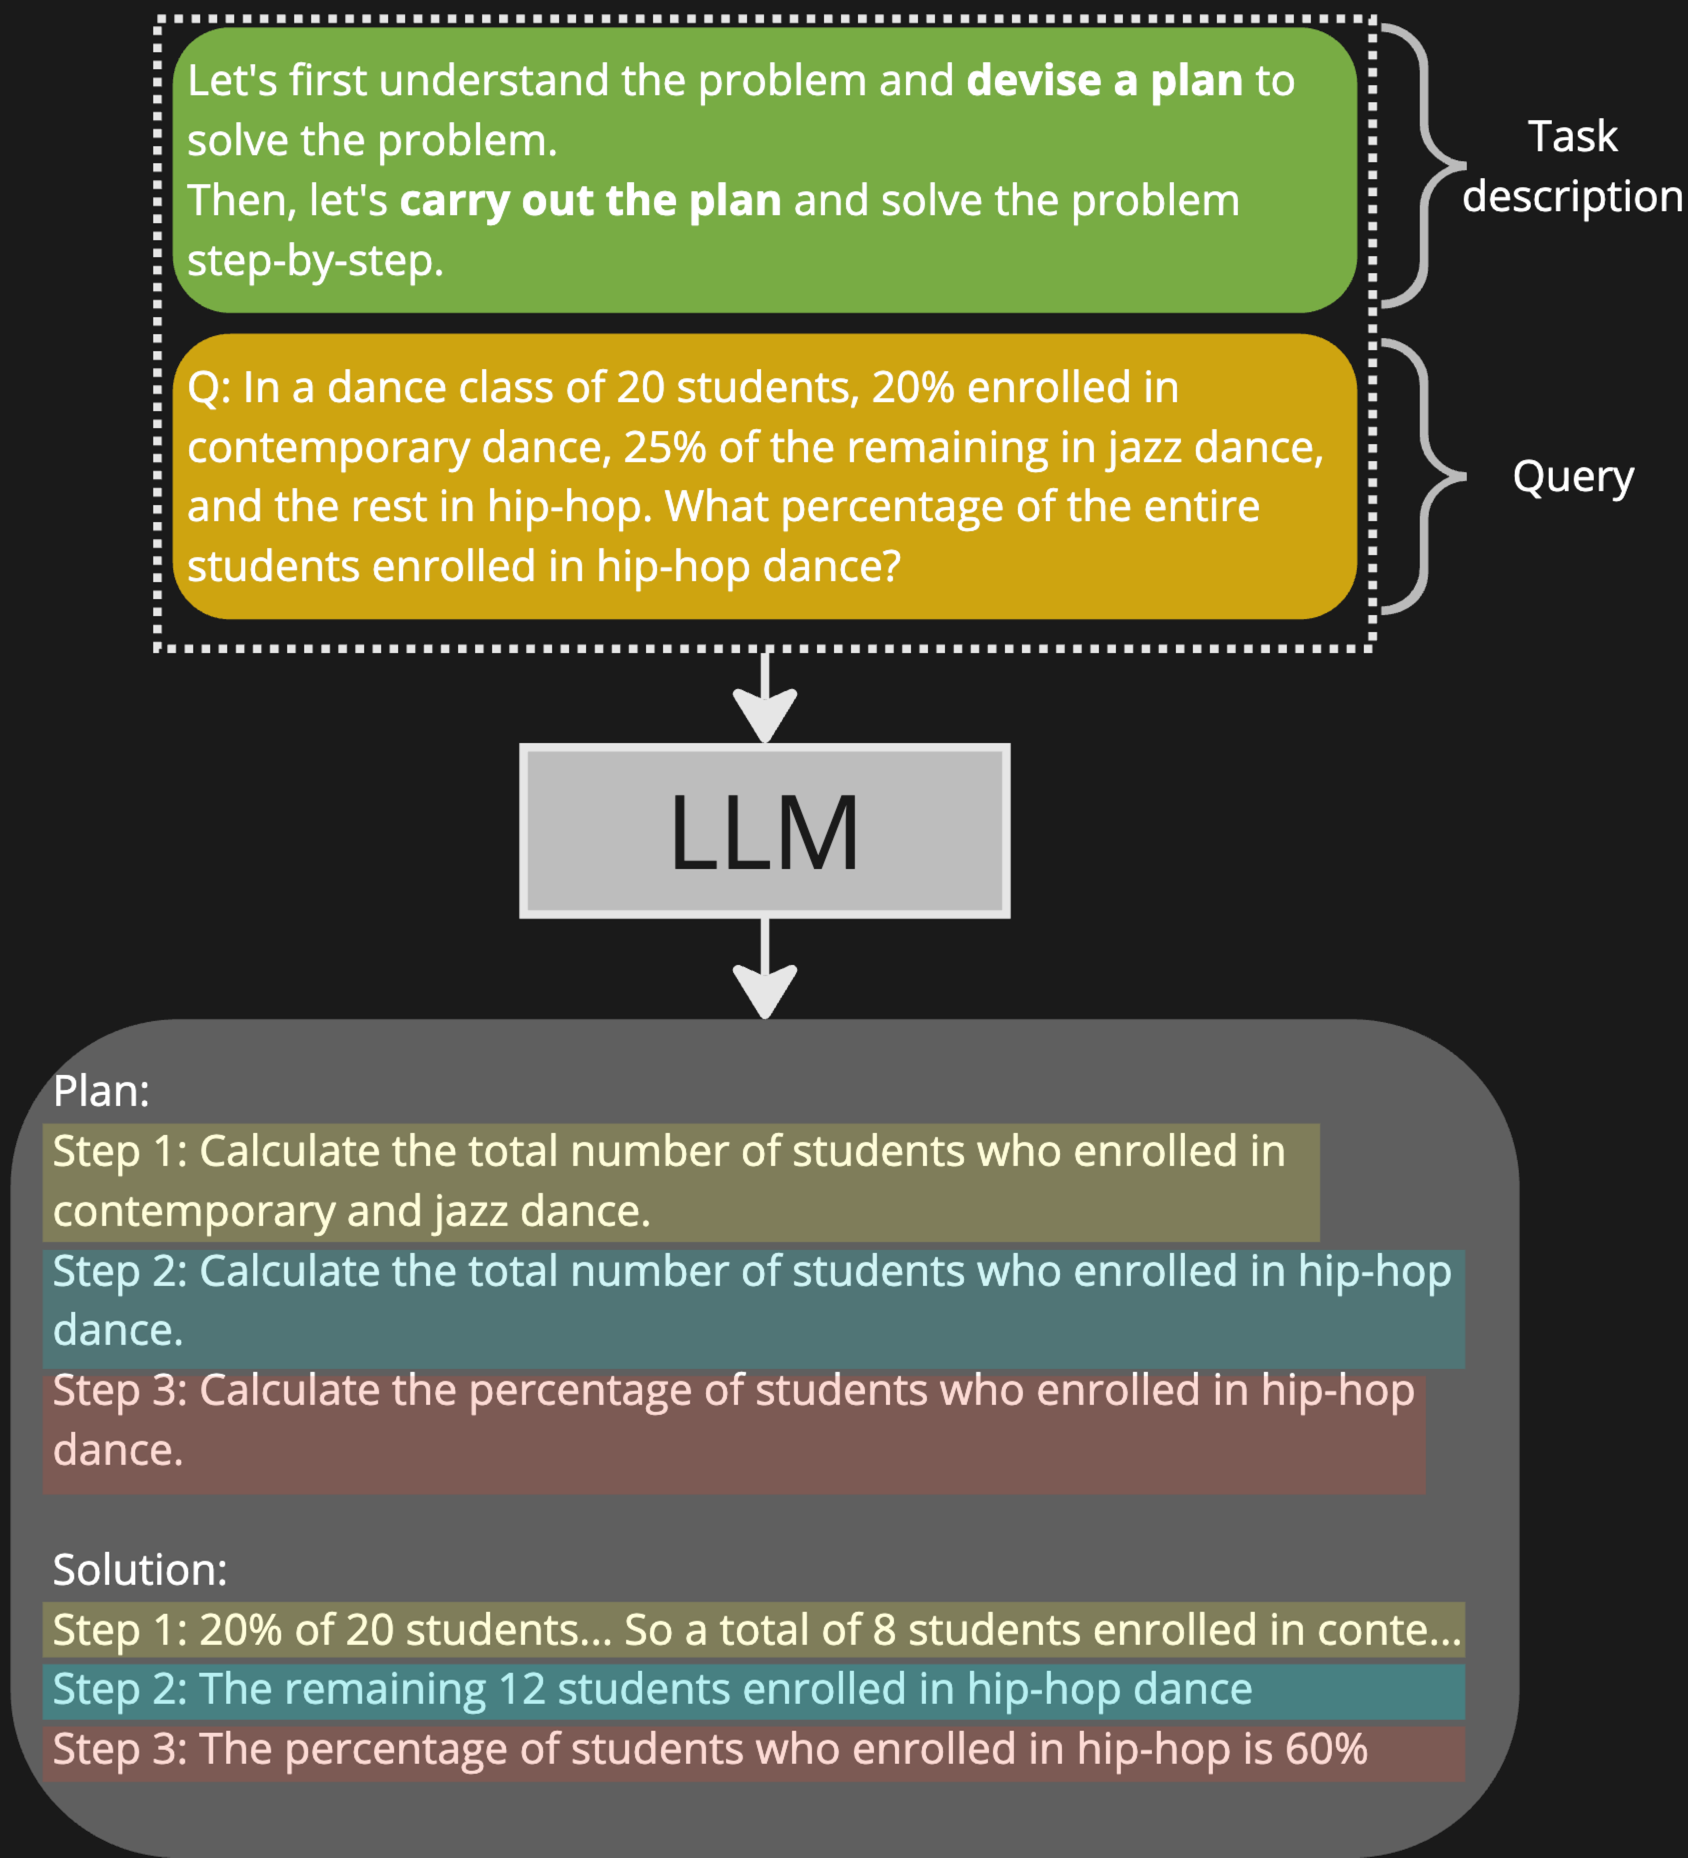
\includegraphics[width=0.8\textwidth]{planning}
	\caption{The general framework of prompt-based planning. Source: \textcite{survey}}
	\label{fig:planning}
\end{figure}

In this paradigm, there are three main components: the planner, the executor, and the environment\footnote{It's similar to Reinforcement Learning, where the planner is the agent, the executor is the policy, and the environment is the world, but the difference is that in RL they are tipically interleaved in the agent, while in prompt-based planning they are separated}.
Specifically the planner, which is a LLM, generates a plan of actions to solve a task.
The plan can be generated in various forms, .e.g., natural language, symbolic, or programmatic~\cite{gao2023pal, zhou2022least}.
The task planner can be enhanced with the memory mechanism, which can store intermediate results and reuse them in the future.

--add details from cite --

Plan executor is responsible for executing the plan generated by the planner.
It can be implemented as a separate LLM for textual tasks, or as a program executor for programmatic tasks~\cite{wang2023plan, gao2022pal}.

Environment is the world where the task is executed, which can be set up as the LLm itself, or an external system, e.g., a simulator or a virtual world likeMinecraft~\cite{yao2023tree, wang2023voyager}.
The environment provides feedback to the task planner about the result of the actions, which can be used to update the plan, either in form of natural language or from other multimodal signals~\cite{shinn2023reflexion, lu2023multimodal}

-- just to add some text --

For solving complex tasks, the planner needs to generate a plan that is long-term and multi-step, which requires the planner to have the ability to reason over long-term dependencies and to generate a plan that is coherent and consistent.
It first need to understand the task and break it down into sub-tasks, then generate a plan that can accomplish the task by executing the sub-tasks in a proper order (see Section~\ref{subsec:plan-generation}).
The plan should be generated in a way that is interpretable and executable by the executor, which acts according to the plan and interacts with the environment to accomplish the task (see Section~\ref{subsec:plan-execution}).
The planner can further incorporate the feedback from the environment to update the plan and refine it to achieve better performance (see Section~\ref{subsec:plan-refinement}).

\subsection{Plan generation}
\label{subsec:plan-generation}

\subsection{Plan execution}
\label{subsec:plan-execution}

\subsection{Plan refinement}
\label{subsec:plan-refinement}